\documentclass[12pt,fleqn]{article}
\usepackage{a4wide}
\usepackage[czech]{babel}
\usepackage[utf8]{inputenc}
% \usepackage[utf8]{inputenc}   % pro unicode UTF-8
% \usepackage[cp1250]{inputenc} % pro win1250
\usepackage{amsmath,amsfonts,amssymb,amsthm}
\usepackage{multicol}
\usepackage[a4paper]{geometry}
\geometry{top=25mm, bottom=25mm, left=25mm, right=25mm}
%\usepackage{indentfirst}    % odsazení prvního řádku v prvním odstavci
\usepackage{color}%kvůli barvám ČVUT
\usepackage[pdftex]{psfrag,graphicx}
\usepackage{pdflscape} %otaci stranky
\usepackage{fancyvrb}
\usepackage{fancyhdr}
\renewcommand{\headrulewidth}{0pt}
% zahlavi vlevo
\lhead{}
% zahlavi vpravo
\rhead{}
% zapati vlevo
\lfoot{PRA ZS 2014/2015}
% zapati uprostred
\cfoot{\thepage}
% zapati vpravo
\rfoot{\copyright \ Adéla Pospíšilová}
% nastavime pouziti toho stylu
\pagestyle{fancy}
%\usepackage{multicol}
%\usepackage{ulem} % podtrhava text pomoci uline, uuline, uwave, ...
\parskip=4pt
\parindent=0pt % neodsazovat první řádek
\newcommand{\HRule}{\rule{\linewidth}{0.1mm}}
\usepackage{wasysym}
\usepackage{MnSymbol}
\usepackage{hyperref}
\usepackage{wrapfig}

\begin{document}
\section*{Návod na namodelování 2D prutovou konstrukci v~programu EduBeam}

EduBeam je univerzitní projekt, jehož cílem je vytvořit jednoduchý, snadno ovladatelný program pro základní analýzu rámových konstrukcí. V současné době umožňuje analýzu 2D rámových konstrukcí v grafickém prostředí. Hlavním cílem je nabídnout studentům jednoduché prostředí pro výpočty metodou konečných prvků, které mohou sami snadno rozšiřovat, využít své znalosti, naučit se nenásilně programovat a přispět k rozvoji tohoto projektu.

Program EduBeam si můžete stáhnout na stránce \url{http://www.oofem.org/wiki/doku.php?id=edubeam:edubeam}. Pokud používáte Windows, pak doporučuji stáhnout aktuální verzi (v době psaní tohoto dokumentu byla nejnovější verze 3.3.0) pro MS Windows (XP, 7 ...). Program je ozkoušen i na systému Windows 8.1.

Při otevření programu EduBeam 3.3.0 vyskočí úvodní obrazovka a v ní klikneme v horní liště na Upravit, kde budeme postupně používat všechny položky (viz obrázek \ref{fig:EduBeam_upravy}). Pokud by se nám něco nepodařilo zadat správně, pak použijeme v nabídce Upravit Upravit nebo eventuelně smazat.

\begin{figure}[ht]
\centering
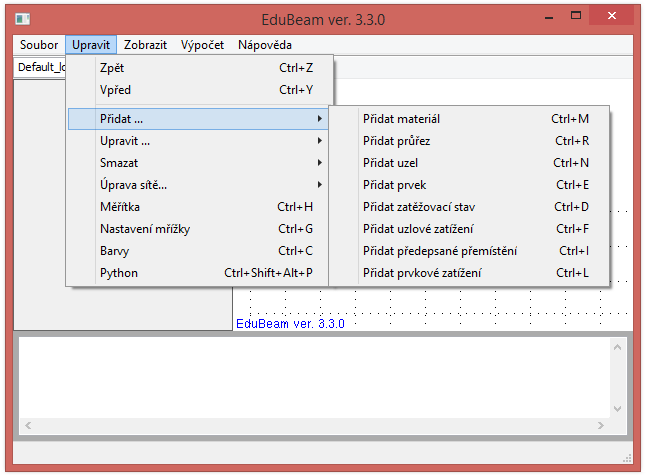
\includegraphics[width=0.99\textwidth]{figs/eduBeam_upravy.png}\caption{Program EduBeam a položky v liště Upravit}\label{fig:EduBeam_upravy}
\end{figure}

Po zadání veškterých vstupních hodnot klikneme na Výpočet a Výpočet úlohy a ve Výpočet v PostProcesoru zobrazíme požadované výsledky zakliknutím v menu na levé straně. Pokud by nám překáželo zatížení na konstrukci, pak ho vypneme pomocí Zobrazit a odtržením položky Zobrazit zatížení. Posouvat konstrukci můžeme pomocí zmáčknutí kolečka na myši, jeho držení a posouvání obrazu. Zvětšování a zmenšování modelu je možné pomocí rolování kolečkem.

\subsection*{Příklad}

Pro výpočet vnitřních sil v 10. domácím cvičení lze využít tento program a za malou chvíli získat vykreslení vnitřních sil. Jako zadání modelu bude využita konstrukce ze vzorového řešení.

\begin{figure}[ht]
\centering
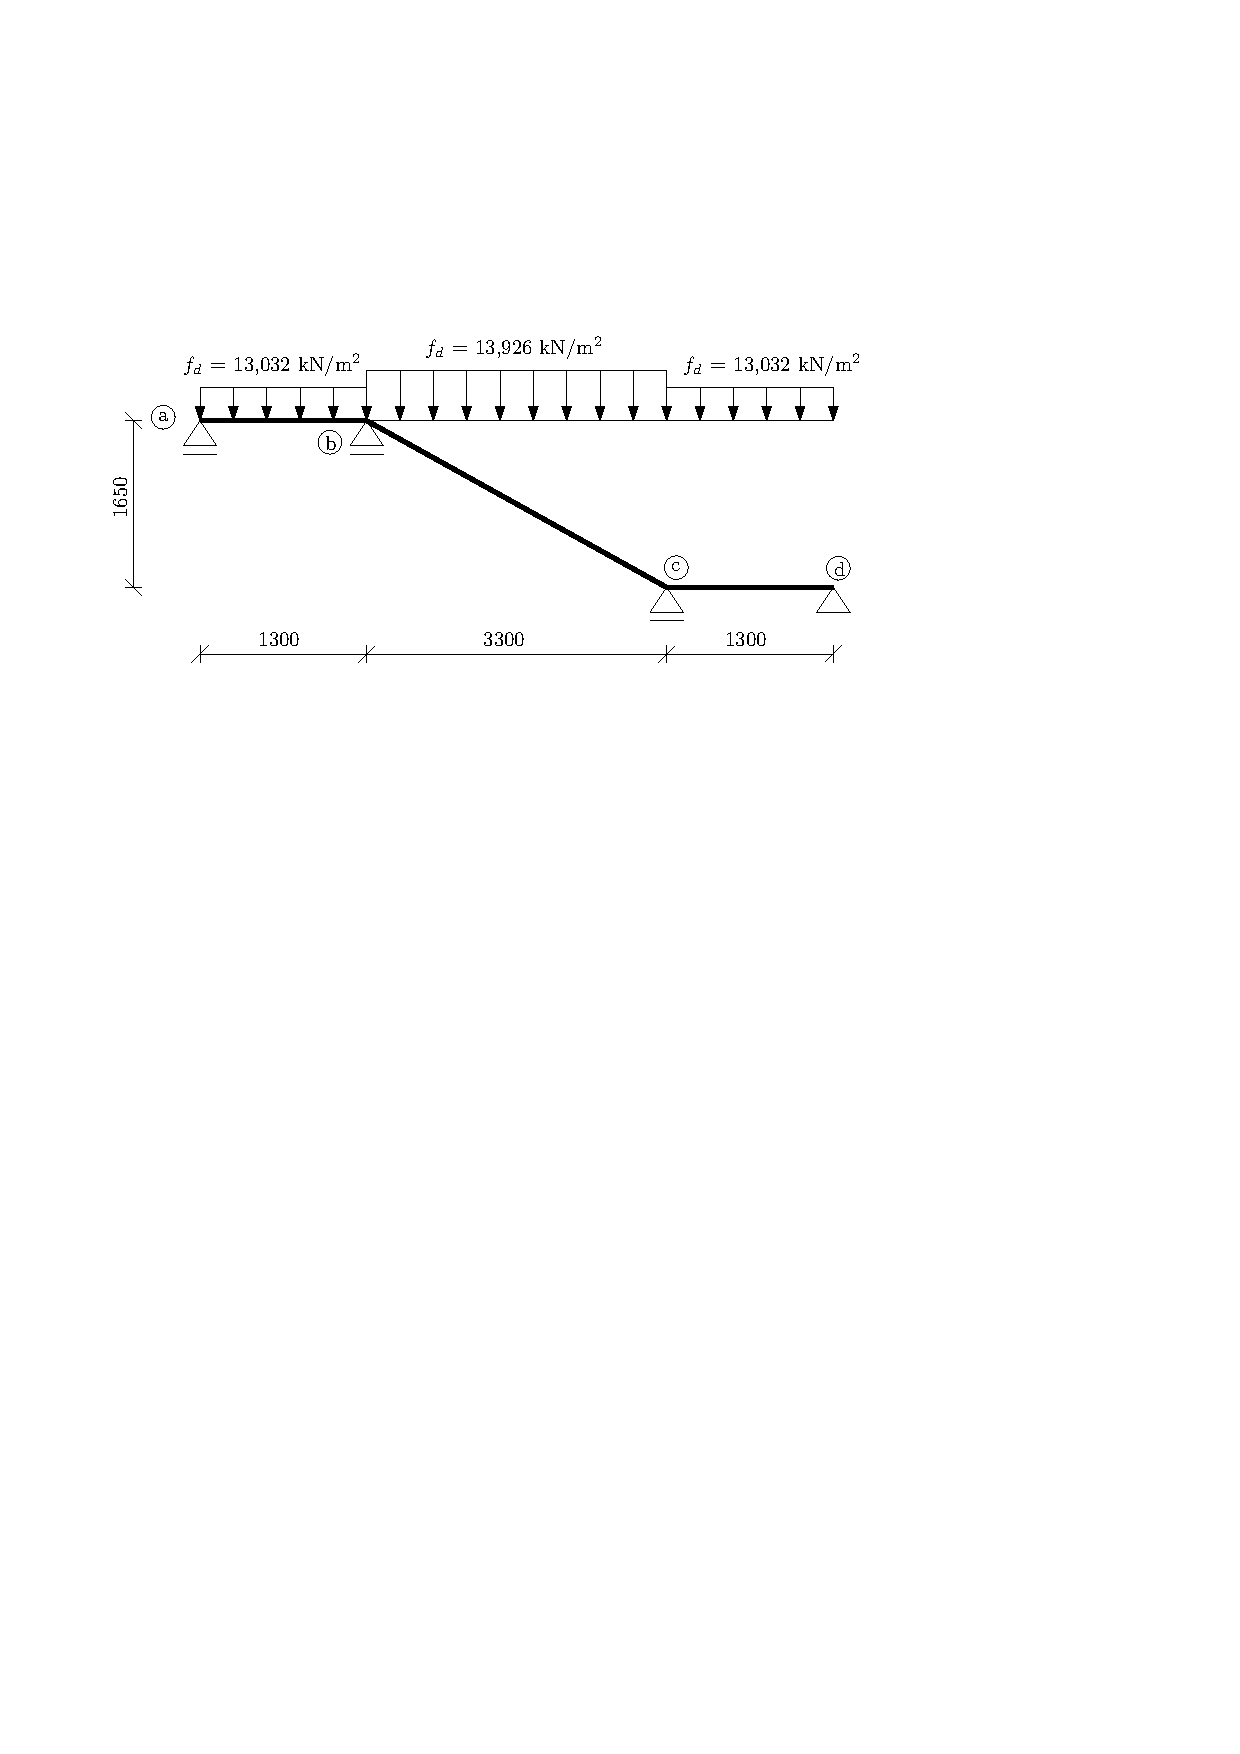
\includegraphics[width=0.99\textwidth]{figs/zadani.pdf}
\end{figure}

V položce Upravit a Přidat \emph{přidáme materiál}. Schodiště je betonové, předpokládáme beton C25/30, který má $E_{cm}$ = 30,5 GPa. Proto hodnotu modulu pružnosti v defaultním materiálu můžeme ponechat. Pokud ovšem budete mít materiál specifikovaný, pak samozřejmě zadávejte skutečnou hodnotu modulu pružnosti. Hodnota modulu pružnosti je potřeba zadávat u výpočtu vnitřních sil pouze u staticky neurčitých konstrukcí, u staticky určitých jsou vnitřní síly na modulu pružnosti nezávislé. Pro výpočet posunů je ale nutné tuto hodnotu zadat, ať už je konstrukce staticky určitá nebo neurčitá (viz cvičení z předmětu PRA). Pokud nebudeme uvažovat žádné teplotní zatížení, pak koeficient teplotní roztažnosti $\alpha$ nebude výpočet ovlivňovat a tudíž můžeme tuto hodnotu taktéž ponechat. Všimněte si ale, že přednastavená hodnota součinitele teplotní roztažnosti je defautně zadaná pro beton (a stejná je i pro ocel). Pokud parametry materiálu měníme, pak klikneme na přidat, pokud vystačíme s přednastavenými, pak se posuneme do další nabídky v Upravit a Přidat.

\begin{wrapfigure}[13]{r}{200pt}
\begin{center}
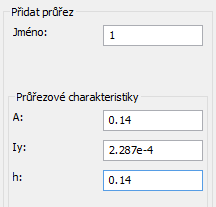
\includegraphics[width=0.3\textwidth]{figs/eduBeam_prurez.png}\caption{Přidání průřezu v programu EduBeam.}\label{fig:EduBeam_pridatprurez}
\end{center}
\end{wrapfigure}
Nyní je na čase \emph{přidat průřez}. Na papíře bokem si musíme spočítat plochu průřezu A a~moment setrvačnosti Iy. Výška průřezu je zde označena jako h. Pokud budete chtít vykreslovat vnitřní síly v kN, kNm a posuny v metrech, pak zadávejte v průřezu všechny průřezové charakteristiky v mocninách metru. Uvažujeme průřez vysoký 0,140 m a široký 1 m. Plocha průřezu A je tedy rovna 0,140 m$^2$ a moment setrvačnosti Iy je roven $2,287 \cdot 10^{-4}$ m$^4$, kterou můžeme zadat jako 2.287e-4. Výška průřezu h je rovna 0,140 m. Zadání v programu viz obrázek~\ref{fig:EduBeam_pridatprurez}. Všimněte si, že se v programu používá desetinná tečka! Pro zadání průřezu do programu klikneme na Přidat.

Nyní přidáme \emph{uzly konstrukce}. V nabídce Upravit a Přidat zvolíme přidat uzel. Uzly přidáváme všude, kde jsou na konstrukci podpory, mění se geometrie průřezu nebo topologie konstrukce, případně tam, kde je na konstrukci bodová síla nebo kde chceme zdát hodnotu vnitřní síly nebo přemístění (posunů, průhybů nebo pootočení). Pro každý přidaný průřez můžeme předepsat okrajové podmínky u, w a r. Pokud je okénko zaškrtnuté, pak je zabráněno posunu v příslušném směru (u nebo w) nebo pootočení (r). \textbf{Vetknutí} tedy namodelujeme zaškrtnutím všech okének (zabráněno posunům ve vodorovném i svislém směru a~taktéž pootočení), \textbf{pevný kloub} namodelujeme pomocí zaškrtnutí okénka u a v, \textbf{posuvný kloub volně klouzající ve vodorovném směru} (tak, jak je v zadání) namodelujeme pomocí zaškrtnutí okénka v (zabraňujeme posunu ve svislém směru), \textbf{posuvný kloub volně klouzající ve svislém směru} modelujeme pomocí zaškrtnutí okénka u. \textbf{Posuvné vetknutí} modelujeme zaškrtnutím jednoho posunu (u nebo v, podle orientace v~zadání) a pootočení r. Souřadnice uzlů můžeme zadávat buď myší a sledováním souřadnic v levé nabídce pro přidání uzlu nebo souřadnicemi. Každý přidaný uzel přidáme do programu pomocí tlačítka Přidat. Program EduBeam má orientovanou osu z svisle dolů, proto při zadávání souřadnic s tímto počítejte, viz obrázek~\ref{fig:EduBeam_uzel}.

\begin{figure}[ht]
\centering
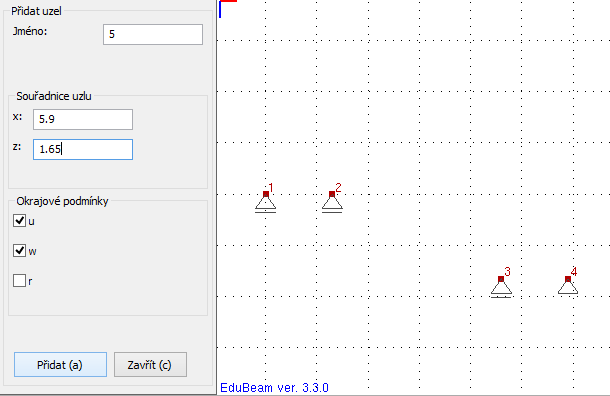
\includegraphics[width=0.99\textwidth]{figs/eduBeam_uzly.png}\caption{Přidání uzlu v programu EduBeam.}\label{fig:EduBeam_uzel}
\end{figure}

Po zadání uzlů se posuneme k \emph{přidání prutů}. V nabídce Upravit a Přidat vybereme Přidat prvek. Vybereme vždy počáteční a konzový uzel, vybereme i příslušný materiál a průřez a zvolíme, jestli je na konstrukci vnitřní kloub na počátku nebo na konci prutu. Náš nosník je jednoduchý lomený nosník (není to složená konstrukce), proto žádné klouby vkládat nebudeme. Pokud byste modelovali příhradovou konstrukci, pak musíte na počet prutů ve styčníku - 1 přidat vnitřní klouby. Pokud by na konstrukci byl jeden dvojný kloub, pak na libovolně zvolený prut přidáte jeden vnitřní kloub (ve styčníku s vnitřním kloubem by tedy byl jeden prut s kloubem a jeden prut bez něj). Jelikož jsme nechali původní materiál jako vyhovující, pak u prutů vždy vybíráme DefaultMat, průřez jsme zadali pouze jeden, čili pro všechny pruty vybíráme průřez 1. Pokud jsme zadávali styčníky zleva doprava, pak postupně zadáme pruty 1 až 3 s počátečními a koncovými uzly 1-2, 2-3, 3-4. Nezapomeňte každý přidávaný prut potvrdit tlačítkem Přidat. Zadání prutů viz obrázek~\ref{fig:EduBeam_prvek}.

\begin{figure}[ht]
\centering
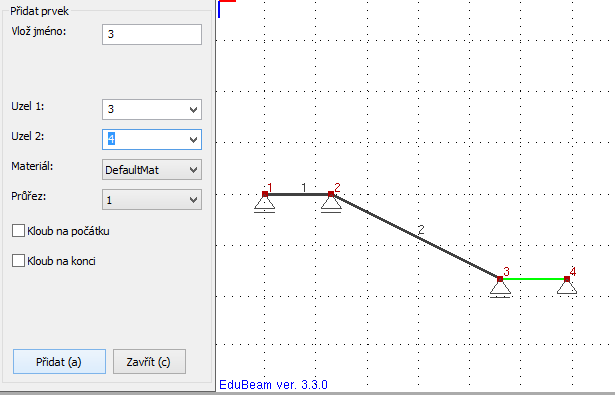
\includegraphics[width=0.99\textwidth]{figs/eduBeam_prvky.png}\caption{Přidání prvku v programu EduBeam.}\label{fig:EduBeam_prvek}
\end{figure}

Topologii konstrukce máme namodelovanou a posuneme se do přidání zatěžovacích stavů. Jelikož se většinou konstrukce posuzuje na víc zatěžovacích stavů, bylo by složité zadávat pokaždé novou topologii konstrukce. Je jednodušší zvolit více zatěžovacích stavů a pro každý zatěžovací stav mít vypočítané vnitřní síly. My máme jeden zatěžovací stav (návrhové zatížení), zatěžovací stav bude stačit jeden. Pokud byste si chtěli zkontrolovat posuny a tedy maximální průhyb, pak přidejte zatěžovací stavy dva, jeden pro návrhové a jeden pro charakteristické zatížení. Program neuvažuje zatížení vlastní tíhou (nikde se nezadávala objemová hmotnost materiálů), proto vlastní tíhu musíte namodelovat vy pomocí spojitého zatížení, které jste si napočítali dle vzorového příkladu na stránkách předmětu. Po zatěžovacím stavu přidáme zatížení. Uzlové zatížení nikde na konstrukci nemáme, proto ho v nabídce Upravit a Přidat přeskočíme. Stejně tak nemáme předepsané přemístění. 

Spojité zatížení budeme modelovat pomocí nabídky Upravit, Přidat a Přidat prvkové zatížení. Zatížení se zadává pomocí globálního souřadného systému. Pokud byste měli na šikmém prutu kolmé zatížení na prut, musíte ho přepočítat do svislého a vodorovného směru. My ale máme pouze svislé zatížení rovnoběžné s osou z hlavního souřadného systému, proto nám přepočet do lokálních směrů nemusí dělat vrásky. Jediný přepočet bude nutný při přepočtu svislého zatížení na délku prutu. Všimněte si, že v zadání příkladu máme zatížení modelováno na průmět šikmého prutu. Do programu je ale potřeba zadat hodnota spojitého zatížení na délku prutu. Výslednice spojitého zatížení na průmět prutu i na délku prutu musí být stejná. Z této myšlenky vyjdeme a vypočítáme hodnotu zatížení
\begin{eqnarray*}
13,926 \cdot 3,3 = \bar{f}_z \cdot \sqrt{3,3^2 + 1,65^2}, \\
\bar{f}_z = 12,4558 \ \textrm{kN/m}.
\end{eqnarray*}
Postupně na všech prutech namodelujeme zatížení ve směru osy z fz. Vždy vybereme příslušný zatěžovací stav (pokud jich modelujeme víc) v roletkovém menu, vybereme prut, zadáme hodnotu a potvrdíme tlačítkem přidat, viz obrázek~\ref{fig:EduBeam_zatizeni}. Ostatní možné hodnoty zadání prvkového zatížení jsou fx (vodorovné spojité zatížení), dTc (ohřátí střednice - viz příklady v 1. a 2. cvičení předmětu PRA) a dTg (změna ohřevu mezi horními a dolními vlákny, v předmětu PRA nebylo probíráno).

\begin{figure}[ht]
\centering
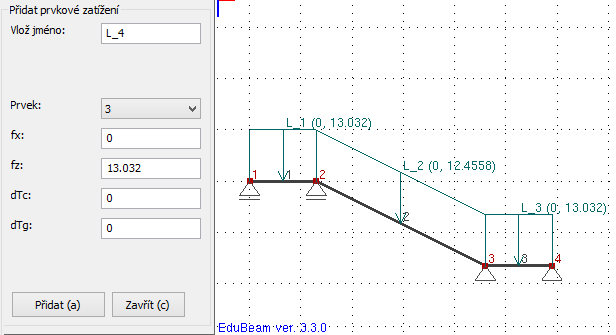
\includegraphics[width=0.99\textwidth]{figs/eduBeam_zatizeni.png}\caption{Přidání prvkového zatížení v programu EduBeam.}\label{fig:EduBeam_zatizeni}
\end{figure}

Konstrukce včetně zatížení je namodelovaná a můžeme tedy pustit výpočet. V horní nabídce vybereme položku Výpočet a v ní zvolíme Výpočet úlohy. Jelikož je úloha jednoduchá, výpočet bude trvat velmi krátce. Po dokončení výpočtu se nám zobrazí úplně dole ve výpisech úkonů uživatele a programu "Úloha úspěšně vyřešena.". Pokud by konstrukce byla namodelovaná špatně, pak je třeba změnit zadání a EduBeam by nám tuto skutečnost oznámil. V nabídce Výpočet ještě klikneme na Postprocesor a zde si vybereme příslušné vnitřní síly, které potřebujeme vykreslit. Pokud nám překáží zatížení, pak ho vypneme pomocí Zobrazit a Zobrazit zatížení.


\vspace{2em}

\textbf{Prosba} V případě, že v textu objevíte nějakou chybu nebo
budete mít námět
na jeho vylepšení, ozvěte se prosím na adela.pospisilova@fsv.cvut.cz. \\ \\






%\end{multicols}
\end{document}